下の図はRuss Cox Blogの中の一文で紹介されているGoデータ構造の文章です。これらの基本型は低レイヤでメモリを分配し、対応する値を保存していることが見て取れるとおもいます。

\begin{figure}[H]
  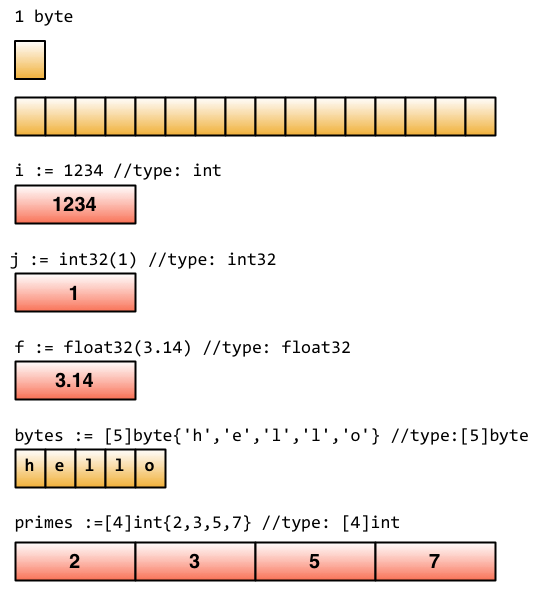
\includegraphics[width=14cm]{2.2.basic.png}
   \label{図2.1}
   \caption{Goデータ形式の保存}
\end{figure}
